\chapter{Approach} \label{ch_approach}
The previous chapter introduced the Nielsen transformation, a prefix-based method to solve the satisfiability problem for unconstrained word equations, and Brzozowski's regex derivatives, a prefix-based method for regex matching. In this chapter, we present our approach of bringing both methods together, effectively extending the Nielsen transformation with regex derivatives to solve the satisfiability problem for regex-constrained word equations.

We now restrict the variables $x \in X$ by adding constraints $c(x) \in R(\Sigma)$.
An assignment $\assignment{\cdot}$ must satisfy these constraints. In other words, $\assignment{x} \in c(x)$ for all $x$.
This approach can handle unconstrained variables as well: For any unconstrained variable $x$, set $c(x)$ to be the catch-all regex $\emptyset'$ with $L(\emptyset') = \Sigma^* \setminus L(\emptyset) = \Sigma^*$.

Variables are now selected over (usually strict) subsets of $\Sigma^*$. This has severe consequences, as questions like "can $x$ be empty?", "is there a solution for $x$?" or "can $y$ be a prefix of $x$?" suddenly become non-trivial.

\section{Algorithm} \label{s_algorithm}
We modify Nielsen's algorithm to also cover regex-constrained variables. While some rewrite rules stay the same (i.e. if both sides start with a terminal symbol), a few rules change when moving from unconstrained to regex-constrained variables. This is because unconstrained variables are always \textit{satisfiable} (i.e. a solution exists) and \textit{nullable} (i.e. can be equal to $\varepsilon$), while for constrained variables we now have to add checks. In the sections \ref{ss_nullability} - \ref{ss_y_prefix_x}, we therefore take into account the ways in which constrained variables differ from unconstrained variables. In section \ref{ss_rnt}, we bring them together and present our modified version of the Nielsen transformation.

\subsection{Nullability} \label{ss_nullability}
While unconstrained variables, selected from $\Sigma^*$, are always \textit{nullable}, i.e. they can be empty, this does not hold for regex-constrained variables. 
Consider $x, c(x) = a\:|\:b$. Then $x$ is not nullable, because $\varepsilon \not\in c(x)$. Thus, no assignment $\assignment{\cdot}$ exists with $\assignment{x} = \varepsilon$. We need to take this into account because case \ref{def:nt_xe} of the Nielsen transformation deletes variables without checking for nullability first.


\subsection {Satisfiability}
Unconstrained variables always have some solution within $\Sigma^*$. Constrained variables on the other hand can have \textit{unsatisfiable} constraints. Take for example $x, c(x) = a\&b$. Then, there exists no assignment $\assignment{\cdot}$ with $\assignment{x} \in c(x)$, because $L(c(x)) = L(a) \cap L(b) = \{a\} \cap \{b\} = \{\}$. This breaks the current setup of the Nielsen transformation: Until now we always assumed that whenever we encounter a variable, there exists some value it can take. We need to take into account, that whenever we work with a variable, we have to check it for satisfiability first. This applies to the cases \ref{def:nt_xe} - \ref{def:nt_xy}.

We introduce the satisfiability function $\sigma: R(\Sigma) \rightarrow \{false, true\}$ with $\sigma(p) \Leftrightarrow L(p) \neq \{\}$.

\[
\begin{tabular}{c c c}
    $\sigma(\emptyset)$ & $=$ & $false$ \\
    $\sigma(\lambda)$ & $=$ & $true$ \\
    $\sigma(a)$ & $=$ & $true$ \\
    $\sigma(pq)$ & $=$ & $\sigma(p) \land \sigma(q)$ \\
    $\sigma(p*)$ & $=$ & $true$ \\
    $\sigma(p')$ & $=$ & $unknown$ \\
    $\sigma(p\:\&\:q)$ & $=$ & $\sigma(p) \land \sigma(q)$ \\
    $\sigma(p\:|\:q)$ & $=$ & $ \sigma(p) \lor \sigma(q)$ \\
\end{tabular}
\]

For $\sigma(p')$ we cannot determine the satisfiability. Consider the satisfiable regex $a|b$. Its negation $(a|b)'$ is satisfiable, because $aa \in (a|b)'$. Now consider the unsatisfiable regex $a\&b$. Again, its negation $(a\&b)'$ is satisfiable, because $a \in (a\&b)'$. So for these two regular expressions -- one satisfiable, the other unsatisfiable -- both negations are satisfiable. Still, let us consider $(a|b)*$ over the alphabet $\Sigma = \{a, b\}$. Then $L((a|b)*) = \Sigma^*$ and subsequently $L(((a|b)*)') = \{\}$, so the negation is unsatisfiable. The satisfiability of the negation $p'$ can therefore not be inferred from the satisfiability of $p$. To be safe, we assume that $p'$ is always satisfiable: $\sigma(p') = true$. Note, that this does not lead to incorrect results: A variable wrongly declared as satisfiable can only be deleted from the word equation later on, if it matches $\varepsilon$ and is therefore satisfiable.

\subsection{$a$ as a prefix of $x$}
If we now encounter case \ref{def:nt_xa} of the Nielsen transformation, i.e. $x\alpha = a\beta$, we assume that $x$ has the prefix $a$. For unconstrained variables this is always possible. For constrained variables we first need to find out if $x$ is allowed to start with $a$. In other words, we need to check that $\sigma(D_a(c(x))$. When rewriting with $\varphi_{x \rightarrow ax'}$, we also need to introduce the new constraint for $c(x') = D_a(c(x))$. If we recycle variable names, we update the constraint $c(x)$ instead.

\subsection{$y$ as a prefix of $x$} \label{ss_y_prefix_x}
For unconstrained variables, things are simpler: $y$ can always be a prefix of $x$.
For regex-constrained variables, it is not trivially possible to check whether one can be another variable's prefix because we have no simple way of finding out if $c(x)$ can begin with some $w \in L(c(y))$. We work around this issue by reformulating it. $y$ can be a prefix of $x$ if it is either empty (i.e. $y = \varepsilon$), or if $x = ax', y = ay'$ and $y'$ is a prefix of $x'$ for some $a \in \Sigma$. The case $y = \varepsilon$ can be safely disregarded because it is already covered in case \ref{def:nt_xe} of the Nielsen transformation. The other case just fixes a shared prefix $a$ for both variables and postpones the rest of the prefix problem for a later step of the Nielsen transformation.
For this to work, both $x$ and $y$ need to be allowed to start with $a$, in other words $\sigma(D_a(c(x))) \land \sigma(D_a(c(y)))$ needs to hold.

As we are interested in finding all $a \in \Sigma$ that fulfill this constraint, we define the prefix-function $\pi: R(\Sigma) \rightarrow 2^\Sigma, \pi(p) = \{a \in \Sigma\:|\:\sigma(D_ap)\}$ that can be algorithmically computed as follows:

\[
\begin{tabular}{c c l}
    $\pi(\lambda)$ & $=$ & $\{\}$ \\
    $\pi(\emptyset)$ & $=$ & $\{\}$ \\
    $\pi(a)$ & $=$ & $\{a\}$ \\
    
    $\pi(pq)$ & $=$ & $
        \left\{
    	\begin{array}{ll}
    		\pi(p) \cup \pi(q)  & \mbox{if } \nu(p) \\
    		\pi(p) & \mbox{if } \neg \nu(p)
    	\end{array}
        \right.
    $\\
    
    $\pi(p*)$ & $=$ & $\pi(p)$ \\
    $\pi(p')$ & $=$ & $unknown$ \\
    $\pi(p\:\&\:q)$ & $=$ & $\pi(p) \cap \pi(q)$ \\
    $\pi(p\:|\:q)$ & $=$ & $\pi(p) \cup \pi(q)$ \\
\end{tabular}
\]

For $\pi(p')$ we cannot determine the possible prefixes, so instead we say any symbol is possible and define $\pi(p') = \Sigma$.

For all $a \in \pi(c(x)) \cap \pi(c(y))$ (and those can be linearly many), we replace $y$ with $ay'$ by use of $\varphi_{y \rightarrow ay'}$ and introduce the new constraint $c(y') = D_a(c(y))$. It suffices to only cover $y = ay'$ and leave out $x = ax'$, because the resulting word equation $x\varphi_{y \rightarrow ay'}(\alpha) = ay'\varphi_{y \rightarrow ay'}(\beta)$ starts with $x$ and $a$ and thus triggers case \ref{def:nt_xa} immediately.

Note, that strictly speaking $\pi$ is not needed. Instead of iterating over $a \in \pi(c(x)) \cap \pi(c(y)) \subset \Sigma$, we could iterate over all $a \in \Sigma$ because unsatisfiable derivatives get filtered out later anyways. For large alphabets $\Sigma$ this comes with a blowup linear in $|\Sigma|$ for every application of case \ref{def:nt_xy}. This accumulates to an exponential blowup for repeated applications of case \ref{def:nt_xy}. We try to minimize this blowup by using $\pi$. This blowup does not exist in the unconstrained version of the Nielsen transformation. It is only introduced by our method of fixing shared prefixes $a$.

\subsection{Modified Algorithm} \label{ss_rnt}
To accommodate regex-constrained variables, we must modify the case analysis of the Nielsen transformation. We integrate the ideas from the previous chapters into the four cases \ref{def:nt_xe} - \ref{def:nt_xy} that deal with variable changes. The two non-terminal cases \ref{def:nt_aa} and \ref{def:nt_ab} stay the same. The updated case analysis looks like this:

Let $a, b \in \Sigma, a \neq b$ be two distinct terminals, $x, y \in X, x \neq y$ two distinct variables with constraints $c(x), c(y) \in R(\Sigma)$ and $\alpha, \beta \in (\Sigma \cup X)^*$ two (possibly equal) strings. Then for the Nielsen transformation, there are the following cases:

\begin{enumerate}
    \item \label{rnt_aa}
        Both sides start with the same terminal: $a\alpha = a\beta$. \\
        We can eliminate this terminal and reduce the equality problem to $\alpha =\beta$.
    
    \item \label{rnt_ab}
        Both sides start with a different terminal: $a\alpha = b\beta$ \\
        The strings cannot be equal because $a \neq b$.

    \item \label{rnt_xe}
        One side starts with a variable: $x\alpha = \beta$ \\
        If $x$ is satisfiable and nullable, i.e. if $\sigma(c(x)) \land \nu(c(x))$, we delete $x$ from the equation using $\varphi_{x \rightarrow \varepsilon}$.
        
        \begin{center}
        \begin{tabular}{r c l}
            $x\alpha$ & $=$ & $\beta$ \\    
            $\varphi_{x \rightarrow \varepsilon}(x\alpha)$ & $=$ & $\varphi_{x \rightarrow \varepsilon}(\beta)$ \\
            $\varphi_{x \rightarrow \varepsilon}(\alpha)$ & $=$ & $\varphi_{x \rightarrow \varepsilon}(\beta)$
        \end{tabular}
        \end{center}

    \item \label{rnt_xa}
        One side starts with a variable, and one starts with a terminal: $x\alpha = a\beta$\\
        If $x$ is satisfiable and if it can start with $a$, i.e. $\sigma(c(x)) \land \sigma(D_a(c(x)))$, we rewrite the equation using $\varphi_{x \rightarrow ax'}$ and we introduce the updated constraint $c(x') = D_a(c(x))$.
        
        \begin{center}
        \begin{tabular}{r c l}
            $x\alpha$ & $=$ & $a\beta$ \\
            $\varphi_{x \rightarrow ax'}(x\alpha)$ & $=$ & $\varphi_{x \rightarrow ax'}(a\beta)$ \\
            $ax'\varphi_{x \rightarrow ax'}(\alpha)$ & $=$ & $a\varphi_{x \rightarrow ax'}(\beta)$ \\
        \end{tabular}
        \end{center}

    \item \label{rnt_xx}
        Both sides start with the same variable: $x\alpha = x\beta$ \\
        If $x$ is satisfiable, i.e. if $\sigma(c(x))$, we delete the prefix $x$ from both sides of the equation leaving us with $\alpha = \beta$.
    
    \newpage
    
    \item \label{rnt_xy}
        Both strings start with different variables: $x\alpha = y\beta$ \\
        We fix a prefix for $y$. For all $a \in \pi(c(x)) \cap \pi(c(y))$, we rewrite using $\varphi_{y \rightarrow ay'}$.
        
        \begin{center}
        \begin{tabular}{r c l}
            $x\alpha$ & $=$ & $y\beta$ \\
            $\varphi_{y \rightarrow ay'}(x\alpha)$ & $=$ & $\varphi_{y \rightarrow ay'}(y\beta)$ \\
            $x\varphi_{y \rightarrow ay'}(\alpha)$ & $=$ & $ay'\varphi_{y \rightarrow ay'}(\beta)$ \\
        \end{tabular}
        \end{center}
\end{enumerate}

The rest of the algorithm stays unchanged: We try to find a directed path from $\alpha = \beta$ to $\varepsilon = \varepsilon$.

\section{Correctness}
\begin{theorem}
The algorithm formulated in \ref{s_algorithm} is correct. A solution for $\alpha = \beta$ exists, iff there is a path from $\alpha = \beta$ to $\varepsilon = \varepsilon$ in the graph of rewrites.
\end{theorem}

\begin{proof}
We will prove both sides of the equivalence separately.

Let $\varphi = \varphi_1 \circ' \varphi_2 \circ' ... \varphi_n$ be the path of rewrites so that $\varphi(\alpha) = \varepsilon = \varphi(\beta)$.

Now, ignore all prefix deletions $\varphi_{DEL}$ and group all rewrites by variable. For each variable $x$ we get $\varphi_x = \varphi_{x \rightarrow ax'} \circ' \varphi_{x' \rightarrow a'x''} \circ' ... \circ' \varphi_{x''' \rightarrow \varepsilon} = \varphi_{x \rightarrow aa'a''...}$. Note, that each $\varphi_x$ must end with $\varphi_{x''' \rightarrow \varepsilon}$, because otherwise $\varphi(\alpha) \neq \varepsilon$ or $
\varphi(\beta) \neq \varepsilon$. 
We define the assignment function $\assignment{x} = \varphi_x(x) = aa'a''...$ and the overall rewrite without prefix deletion $\Phi = \circ'_{x \in X} \varphi_x$ so that $\Phi(\alpha) = \Phi(\beta) \in \Sigma^*$. Then $\alpha = \beta$ holds with the assignment function $\assignment{\cdot}$.
Remember that rewrites of the form $\varphi_{x \rightarrow ax'}$ only exist if $\sigma(D_a(c(x)))$, and $\varphi_{x \rightarrow \varepsilon}$ only exists if $\nu(c(x))$, because otherwise our algorithm does not allow this rewrite. Therefore, $\nu(D_{a'''}(...(D_{a'}(D_a(c(x))))) \Leftrightarrow \varepsilon \in D_{a'''}(...(D_{a'}(D_a(c(x)))) \Leftrightarrow aa'...a''' \in c(x) \Leftrightarrow \assignment{x} \in c(x)$.
It follows that $\alpha = \beta$ has a solution $\assignment{\cdot}$ that satisfies the regex constraints.

Let us now consider the other direction. Let $\assignment{\cdot}$ be the assignment function of a solution for $\alpha = \beta$ that satisfies the regex constraints, i.e. $\assignment{x} \in c(x)$ for all variables $x$. We will now prove there exists a path $\varphi = \varphi_1 \circ' \varphi_2 \circ' ... \varphi_n$ so that $\varphi(\alpha) = \varepsilon = \varphi(\beta)$.

We make a case distinction:
\begin{enumerate}
    \item \label{proof_aa}
    $a\alpha = a\beta$: Both sides start with the same terminal symbol $a$.\\
    We rewrite the equation to $\alpha = \beta$ with $\varphi_{DEL}$ and repeat this case distinction.
    
    \item \label{proof_xe}
    $x\alpha = \beta$: One side starts with the variable $x$ and $\assignment{x} = \varepsilon$. Without loss of generality, we choose the left side.\\
    Note, that $\assignment{x} = \varepsilon$ implies $\nu(c(x))$. We rewrite with $\varphi_{x \rightarrow \varepsilon}$ and repeat this case distinction.
    
    \item \label{proof_xa}
    $x\alpha = a\beta$: One side starts with the variable $x$, the other side starts with the terminal symbol $a$, the assignment $\assignment{x}$ starts with $a$. Without loss of generality we chose the left side.\\
    We rewrite with $\varphi_{x \rightarrow ax'} \circ' \varphi_{DEL}$. Note, that here we have two rewrites because $\varphi_{x \rightarrow ax'}$ results in both sides of the equation starting with $a$. Therefore, we immediately follow up with $\varphi_{DEL}$. Afterwards, we repeat this case distinction.
    
    \item \label{proof_xy}
    $x\alpha = y\beta$: Both sides start with a variable ($x$ and $y$ may be the same), $\assignment{x}$ starts with $a$, $\assignment{y}$ starts with $a$. Note, that this implies $\sigma(D_a(c(x)))$ and $\sigma(D_a(c(y))$. We rewrite with $\varphi_{x \rightarrow ax'} \circ' \varphi_{y \rightarrow ay'} \circ' \varphi_{DEL}$ and repeat this case distinction.
    
    \item \label{proof_ee}
    $\varepsilon = \varepsilon$: The word equation has been fully reduced to $\varepsilon = \varepsilon$. We are done.
\end{enumerate}

This covers all possible cases. Cases like $a\alpha = b\beta$ for $a \neq b$ or $x\alpha = a\beta$ where $\assignment{x}$ does not start with $a$ need not be considered, because they are unsatisfiable and we assumed our word equation to be satisfiable. Furthermore, a rewrite done by the cases \ref{proof_aa} - \ref{proof_xy} always results in another equation that is still satisfiable.

To prove that we ultimately arrive at $\varepsilon = \varepsilon$, we must now only prove that each case moves us closer to $\varepsilon = \varepsilon$. We do this by showing that each case reduces the \textit{complexity} of the word equation.
We define the measure of complexity $||\cdot||$ to be $||\varepsilon|| = 0, ||a|| = 1, ||x|| = |\assignment{x}|+1, ||\alpha_1\alpha_2|| = ||\alpha_1|| + ||\alpha_2||$. We chose this particular definition of complexity solely so that every rewrite reduces the equation's complexity strictly monotonically. Also, this definition ensures that $||\alpha|| = 0 \Leftrightarrow \alpha = \varepsilon$. Let us use the short notation $||\varphi||$ for the change in complexity $\varphi$ achieves:
$||\varphi|| = ||\alpha\beta|| - ||\varphi(\alpha)\varphi(\beta)||$. Note, that $||\varphi_1 \circ' \varphi_2|| = ||\varphi_1|| + ||\varphi_2||$.

Case \ref{proof_aa} reduces the complexity of the word equation, because $||\varphi_{DEL}|| = -2$. Case \ref{proof_xe} also reduces the complexity of the word equation, because $||\varphi_{x \rightarrow \varepsilon}|| \in \{-1, -2\}$ depending on the number of occurrences of $x$. Let us now consider case \ref{proof_xa}. $||\varphi_{x \rightarrow ax'}|| = 0$, because $|\assignment{x'}| = |\assignment{x}| - 1$. Therefore, $||\varphi_{x \rightarrow ax'} \circ' \varphi_{DEL}|| = -2$.
Let us now consider the final case \ref{proof_xy}.
Again, $||\varphi_{x \rightarrow ax'} \circ' \varphi_{y \rightarrow ay'} \circ' \varphi_{DEL}|| = -2$. The only terminating case we can possibly choose is case \ref{proof_ee}. In other words, we only terminate for equations with complexity $0$. This entails that for a solution $\varphi$ with $\varphi(\alpha) = \varepsilon = \varphi(\beta)$ it always holds that $||\alpha\beta|| + ||\varphi|| = 0$.
Keep in mind that the cases \ref{proof_aa} - \ref{proof_xy} reduce the complexity by $1$ or $2$. Therefore, every word equation $\alpha = \beta$ terminates after $k$ iterations where $\frac{||\alpha\beta||}{2} \leq k \leq ||\alpha\beta||$.

\end{proof}

\newpage
\section{Complexity}

\begin{wrapfigure}{l}{0.5 \textwidth} \label{fig:hangup}
\begin{center}
\resizebox{0.4 \textwidth}{!}{
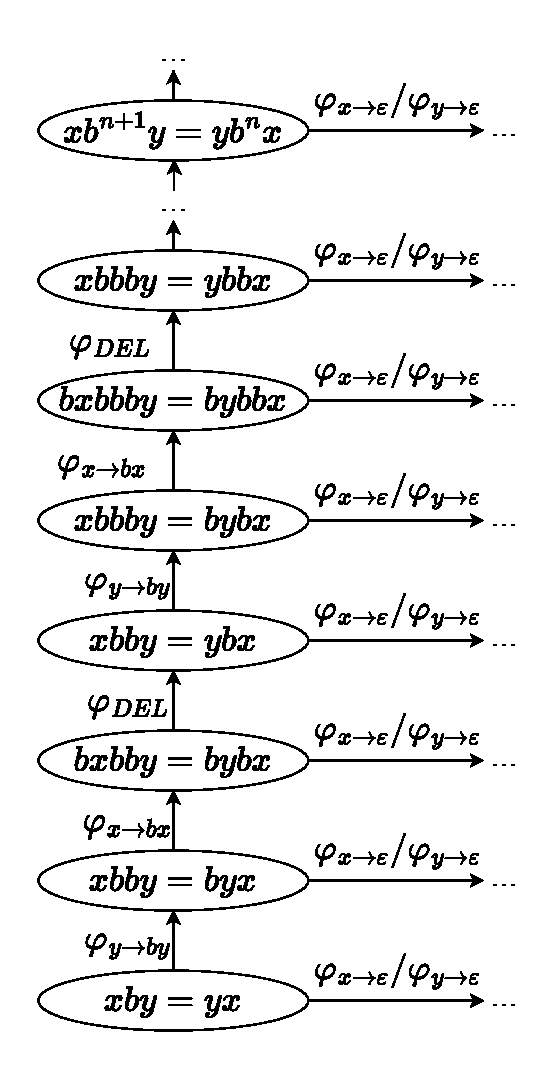
\includegraphics[]{images/xby_yx.pdf}
}
\caption{Graph for the non-terminating word equation $xby = yx, c(x) = (a|b)*, c(y) = b*$}
\label{fig:barplot-2-without-1}
\end{center}
\end{wrapfigure}
The algorithm does not terminate on all unsatisfiable word equations: Consider the equation
$xby = yx, c(x) = (a|b)*, c(y) = (b*)a$. We quickly see that rewriting it with $\varphi_{x \rightarrow \varepsilon}$ or $\varphi_{y \rightarrow \varepsilon}$ does not bring us towards $\varepsilon = \varepsilon$, because the resulting equations $xb = x$ and $by = y$ are dead ends.
Figure \ref{fig:hangup} shows the graph of rewrites. We start in the bottom left with $xby = yx$. We can either delete $x$ or $y$, by rewriting with $\varphi_{x \rightarrow \varepsilon}$ or $\varphi_{y \rightarrow \varepsilon}$, or we fix the shared prefix $b$. If we fix the shared prefix $b$, we trigger the chain of rewrites $\varphi_{y \rightarrow by} \circ' \varphi_{x \rightarrow bx} \circ' \varphi_{DEL}$. This leaves us with the new word equation $xbby = ybx$. The resulting equation again starts with $x$ on the left and $y$ on the right side. We can therefore again fix the prefix $b$. We see that repeating the rewrite chain $\varphi_{y \rightarrow by} \circ' \varphi_{x \rightarrow bx} \circ' \varphi_{DEL}$ for $n$ times gives us the equation $xb^{n+1}y = yb^nx$. We do not reach $\varepsilon = \varepsilon$ and are caught exploring an infinite graph. The algorithm does not terminate.

As we will see in the benchmarks later on, this is an extreme case and a very rare occurrence. Still, we are unable to guarantee that our algorithm terminates on unsatisfiable word equations.

~\\
For satisfiable word equations with a solution $\assignment{\cdot}$, the BFS can be bounded to terminate after $O(||\alpha\beta||)$ iterations. Each node can have $O(|\Sigma|)$ directed neighbors ($O(1)$ for the cases \ref{rnt_aa} - \ref{rnt_xx} and $O(|\Sigma|)$ for case \ref{rnt_xy}). This accumulates to $O(|\Sigma|^{||\alpha\beta||})$ many nodes visited before reaching $\varepsilon = \varepsilon$.

Note, that this does not mean that the satisfiability problem for regex-constrained word equations is undecidable, only that this particular algorithm cannot decide it. We could work around this by making use of regular expression \textit{quotients}.
Let $p, q \in R(\Sigma)$. We define the quotient $p/q$ to be the regular expression describing all words that match $p$ and have a prefix that matches $q$, without that prefix. In other words $L(p/q) = \{w_2\:|\:\exists\:w_1, w_2 \in \Sigma^*, w_1 \in L(q), w_1w_2 \in L(p)\}$. We observe that $D_ap = p/a$. If we can calculate the quotient $p/q$, we can solve the case \ref{rnt_xy} without having to fix a prefix $a$. Instead, when assuming $y$ to be a prefix of $x$, we rewrite with $\varphi_{x \rightarrow yx'}$ and introduce the new constraint $c(x') = c(x)/c(y)$.

\section{Extensibility}
The algorithm described in section \ref{s_algorithm} is agnostic to the regex theory at hand. It does not matter whether we use Brzozowski, Antimirov or transition regexes. The regex theory must only be \textit{derivative-based}, meaning it defines $D, \nu, \sigma, \pi$.

Simple length constraints of the form "$x$ must be of length $k$" can also be expressed as derivative-based constraints. Let $c(x) = k \in \mathbb{Z}$ stand for the constraint that $|\assignment{x}| = k$. Then the definitions

\[
\begin{tabular}{c c c}
    $D_ak$ & $=$ & $k-1$ \\
    $\nu(k)$ & $=$ & $k = 0$ \\
    $\sigma(k)$ & $=$ & $k \geq 0$ \\
    $\pi(k)$ & $=$ & $\Sigma$ \\
\end{tabular}
\]

allow us to integrate length constraints into the algorithm. In this work, although, we will only work with Brzozowski regex constraints.